\documentclass[acmsmall,review,nonacm]{acmart}\settopmatter{printfolios=true,printccs=false,printacmref=false}

\AtBeginDocument{%
	\providecommand\BibTeX{{%
			\normalfont B\kern-0.5em{\scshape i\kern-0.25em b}\kern-0.8em\TeX}}}

\setcopyright{acmcopyright}
\copyrightyear{2018}
\acmYear{2018}
\acmDOI{10.1145/1122445.1122456}

\usepackage{listings}
\usepackage{lipsum}
\usepackage{xcolor}
\usepackage{multirow}


%% These commands are for a PROCEEDINGS abstract or paper.
\acmConference[Woodstock '18]{Woodstock '18: ACM Symposium on Neural
	Gaze Detection}{June 03--05, 2018}{Woodstock, NY}
\acmBooktitle{Woodstock '18: ACM Symposium on Neural Gaze Detection,
	June 03--05, 2018, Woodstock, NY}
\acmPrice{15.00}
\acmISBN{978-1-4503-XXXX-X/18/06}


\begin{document}
	
	\title{Fine-grained Reductions Around CFL Reachability}
	
	\author{Aleksandra Istomina}
	\thanks{Aleksandra Istomina: graduate student, email: aleksandra2999@mail.ru, ACM student member number: 4678238}
	\email{aleksandra2999@mail.ru}
	\affiliation{%
		\institution{Saint Petersburg State University}
		\city{Saint Petersburg}
		\country{Russia}
	}
	\affiliation{%
	\institution{JetBrains Research}
	\city{Saint Petersburg}
	\country{Russia}
	}

    \author{Research advisor: Semyon Grigorev}
    \affiliation{%
    	\institution{Saint Petersburg State University}
    	\city{Saint Petersburg}
    	\country{Russia}
    }
    \affiliation{%
    	\institution{JetBrains Research}
    	\city{Saint Petersburg}
    	\country{Russia}
    }
	
	\newcommand\todo[1]{{\color{violet}#1}}
	\newcommand\db[1]{{\color{red}#1}}
	\newcommand\question[1]{{\color{cyan}#1}}


	\maketitle
	
	\section{Introduction}
	
	\subsection{\todo{brief description of the problem, areas of usage, idea of solution}}
	
	cfpq appears in static code analysis, graph databases, bioinformatics
	
	2npda hard problem
	
	finding valid paths between vertices
	
	\subsection{\todo{problems with current cfpq results}}
	
	several cubic algorithms exist
	
	can we do significantly better? no such algorithm had been found for several decades
	
	maybe we can prove that no such algorithm exist under some hypothesis
	
	\subsection{\todo{main problem}}
	
	fine-grained complexity has some results in the area
	
	results are scattered, have no structure
	
	maybe everything is already proven
	
	\subsection{\todo{main goals, overview}}
	
	collect existing results into easy-to-read form
	
	focus on static, dynamic problems are omitted from this research
	
	state open problems
	
	\section{Preliminaries}
	
	cfg, directed graph, cfl reachability and recognition, note on Dyck-1, fine-grained reduction
	
	\section{Main Results}
	
	\begin{figure}[!htp]
		
		\begin{center}  
			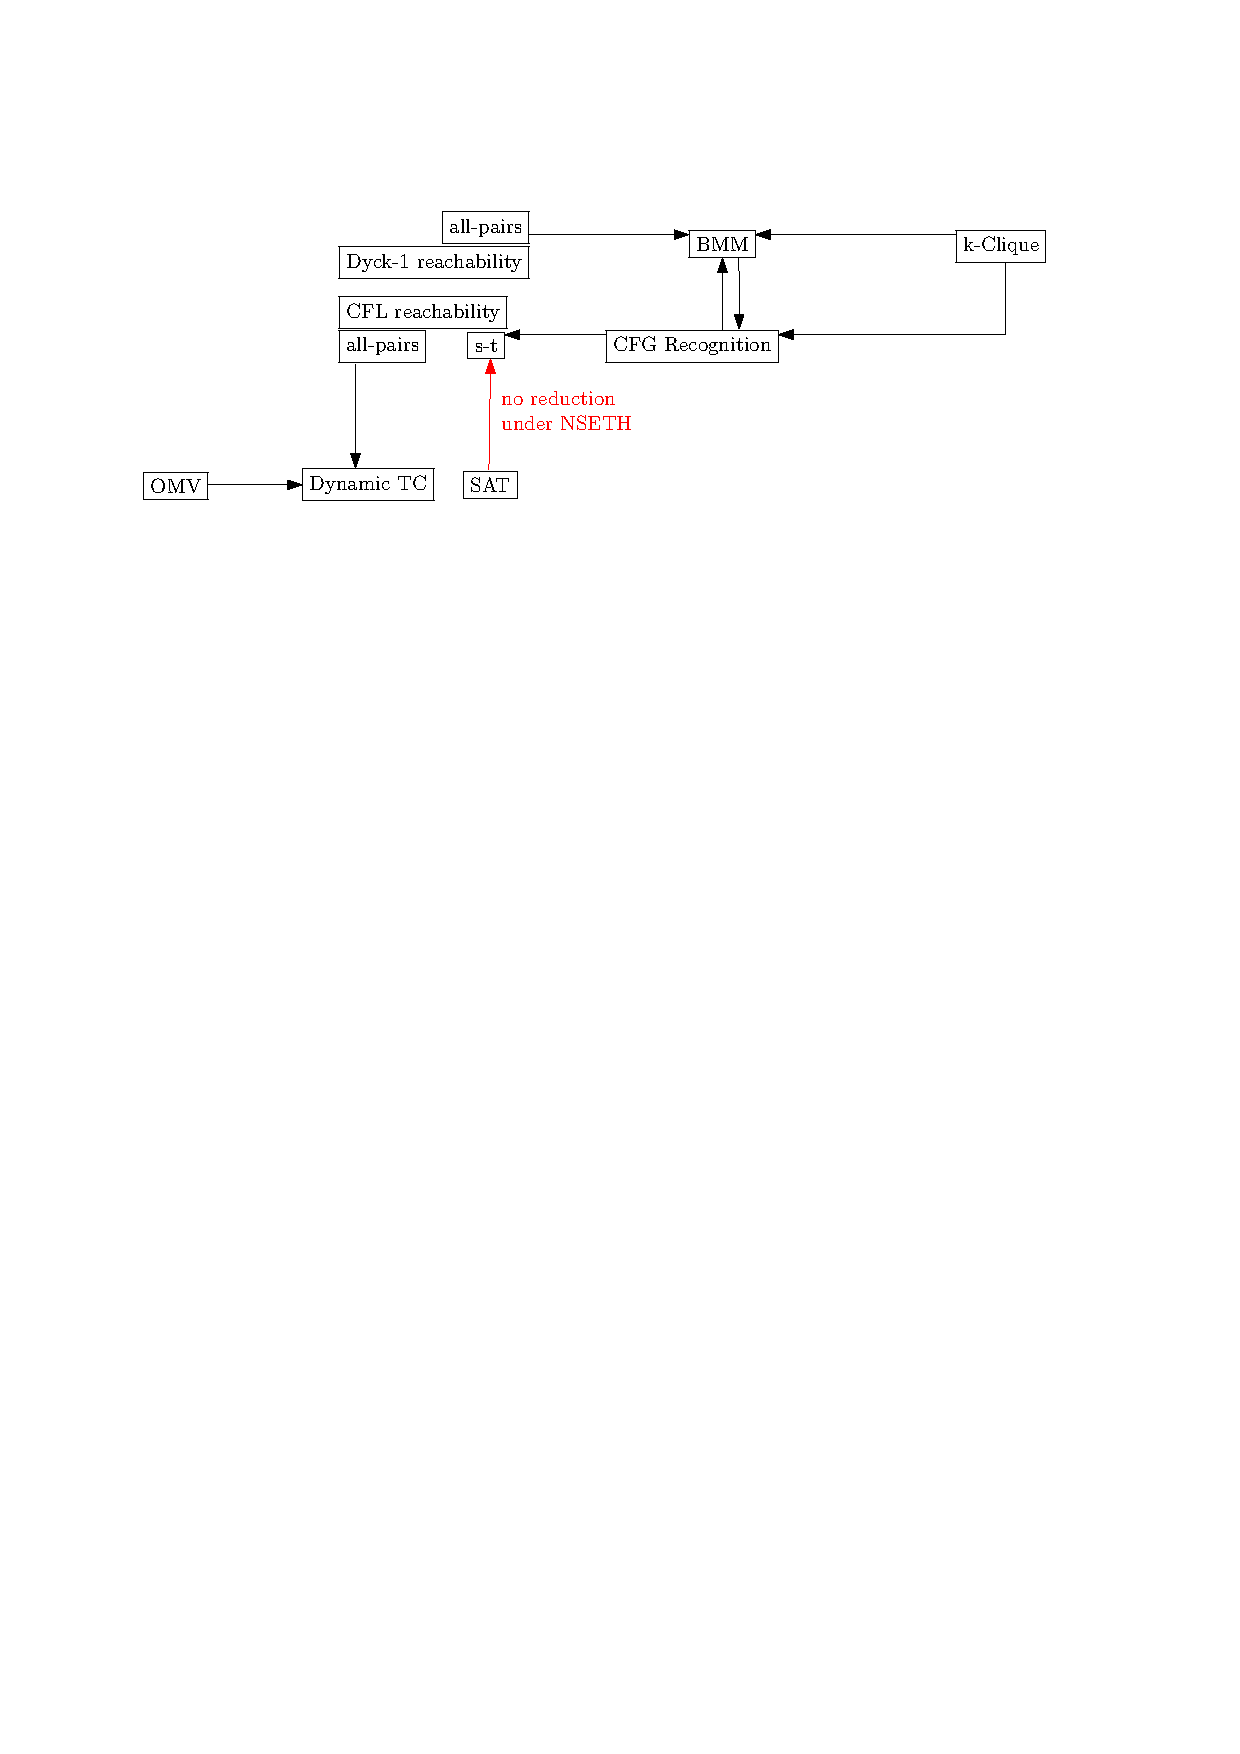
\includegraphics[scale = 0.6]{map_popl.pdf}
		\end{center}
	
		\caption{Black arrow $a \rightarrow b$ represent existing reduction from $a$ to $b$, directions of future work are marked with dashed arrows. Red and turquoise arrows analogously represent non-existence of the reduction and open problems respectively. }
		
	\end{figure}
	
	In \cite{valiant1975general}
	
	\subsection{existing problems and hypotheses}
	
	There are several problems that are connected with CFL Recognition and Reachability. 
	\emph{Boolean satisfiability problem (SAT, $k$-SAT)} determines if there exists an interpretation of variables that satisfies a given Boolean formula on $n$ variables written in $k$-CNF, $k > 3$. The hypothesis about SAT, that we are interested about, is NSETH which proposes that there is no $\epsilon > 0$ such that $k$-SAT can be solved co-nondeterministically in time $2^{(1 - \epsilon) n}$ for any $k$.
	In \emph{Boolean Matrix Multiplication (BMM)} problem it is needed to calculate matrix product of the two given $n \times n$ matrices over (AND, OR). BMM hypothesis states that there is no $\mathcal{O}(n^{3 - \epsilon})$ combinatorial algorithm for that. 
	\emph{Orthogonal Vectors (OV)} problem decides whether the set of $n$ boolean vectors contain two which dot product equals zero. Hypothesis states that OV problem can not be solved in $\mathcal{O}(n^{2 - \epsilon})$ time. 
	Given a context free language $L(G)$ the \emph{Language Edit Distance (LED)} problem seeks the minimum number of edits (insertions, deletions and substitutions) required to convert the given string $s$ into a member of $L(G)$. The fully \emph{dynamic transitive closure (DTC)} problem asks to maintain reachability information in a directed graph between arbitrary pairs of vertices under insertions and deletions of edges.
	
	\subsection{\todo{existing reductions}}
	
	CLFLR <-> SetConstr
		
	dynamic TC to all-pairs
	
	BMM to Dyck-1
	
	s-t -> cfg -> bmm => no combinatorial algorithm
	
	short s-t certificates => no reduction from SAT
		
	\subsection{\todo{open problems}}
	
	This paper is a part of research dedicated to determination of existence or non-existence of a truly subcubic algorithm for CFL Reachability. 
	
	
	There are several reductions that seem promising: reduction from OV to s-t CFL Reachability that 
	
	global: subcubic cfpq
	
	s-t vs all-pairs reachability: comparison with triangles detection problem
	
	ov -> dyck-1
	
	\section{Conclusion and Future work}
	
	subcubic cfpq
	
	reduction form ov, similar to OV -> APA
	
	formalisation of naive reduction LED to s-t
	
	possible reduction form APSP and reformulations
	
	\section{Acknowledgments}
	
	\bibliographystyle{ACM-Reference-Format}
	\bibliography{map}
	
	\appendix
	
\end{document}
\endinput
